%! Author = zero
%! Date = 29/07/2024

% Preamble
\documentclass[a4paper, 12pt]{article}

\usepackage[english,russian]{babel}
\usepackage[T2A]{fontenc}
\usepackage[utf8]{inputenc}
\usepackage{geometry}
\usepackage{enumitem}
\usepackage{setspace}
\usepackage{amssymb}
\usepackage{graphicx}
\usepackage{float}
\usepackage{wrapfig}
\geometry{top=5mm}
\renewcommand{\arraystretch}{1.2}
\linespread{1}

% Document
\begin{document}
    \begin{center}
        \textbf{
            Самостоятельная работа №1\\
            Основы алгебры логики}
    \end{center}

    \begin{enumerate}
        \item $C = 1, D = 1, E = 1, F = 0$

        \item Построить таблицу истинности:
        \begin{enumerate}
            \item $A \vee B \wedge \overline B$\\
            \begin{tabular}{|c|c|c|c|c|c}
                \hline
                $A$ & $B$ & $\overline B$ & $B \wedge \overline B$ & $F$ \\
                \hline
                $0$ & $0$ & $1$           & $0$                    & $0$ \\
                \hline
                $0$ & $1$ & $0$           & $0$                    & $0$ \\
                \hline
                $1$ & $0$ & $1$           & $0$                    & $1$ \\
                \hline
                $1$ & $1$ & $0$           & $0$                    & $1$ \\
                \hline
            \end{tabular}

            \item $(B \vee C) \wedge (\overline A \wedge C \vee \overline C)$\\
            \begin{tabular}{|c|c|c|c|c|c|c|c|c|}
                \hline
                $A$ & $B$ & $C$ & $\overline A$ & $\overline C$ & $B \vee C$ & $\overline A \wedge C$ & $\overline A \wedge C \vee \overline C$ & $F$\\
                \hline
                $0$ & $0$ & $1$ & $1$           & $0$           & $1$        & $1$                    & $1$                                     & $1$ \\
                \hline
                $0$ & $1$ & $0$ & $1$           & $1$           & $1$        & $0$                    & $1$                                     & $1$ \\
                \hline
                $0$ & $1$ & $1$ & $1$           & $0$           & $1$        & $1$                    & $1$                                     & $1$ \\
                \hline
                $1$ & $0$ & $0$ & $0$           & $1$           & $0$        & $0$                    & $1$                                     & $0$ \\
                \hline
                $1$ & $0$ & $1$ & $0$           & $0$           & $1$        & $0$                    & $0$                                     & $0$ \\
                \hline
                $1$ & $1$ & $0$ & $0$           & $1$           & $1$        & $0$                    & $1$                                     & $1$ \\
                \hline
                $1$ & $1$ & $1$ & $0$           & $0$           & $1$        & $0$                    & $0$                                     & $0$ \\
                \hline
            \end{tabular}
        \end{enumerate}

        \item Решить кругами Эйлера:
        \begin{enumerate}
            \item $A \wedge B \vee C$\\


            \item $Z \vee A \wedge C \vee \overline B$\\
        \end{enumerate}

        \begin{figure}[h]
            \centering
            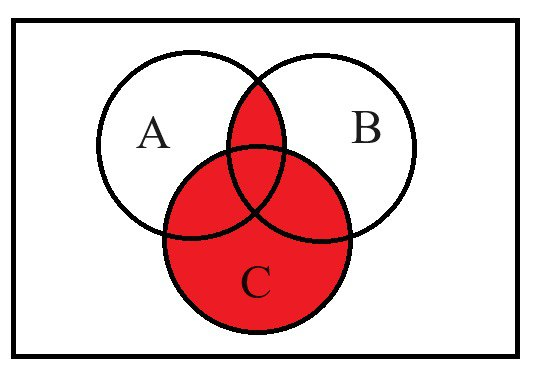
\includegraphics[width=0.2\linewidth]{images/im1}
            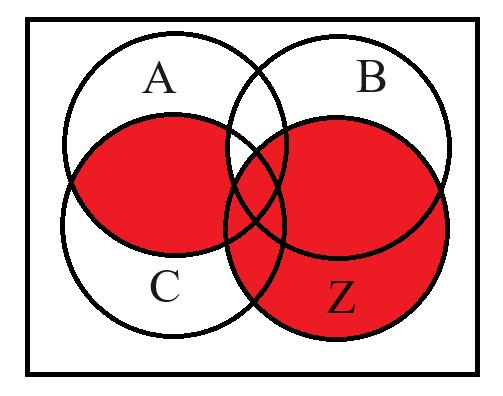
\includegraphics[width=0.2\linewidth]{images/im2}
        \end{figure}

        \item Найти $X, Y$ при которых выражение $X \wedge Y \vee Y = 1$\\
        \begin{tabular}{|c|c|c|c|c|}
            \hline
            $X$ & $Y$ & $X \wedge Y$ & $X \wedge Y \vee Y$\\
            \hline
            $0$ & $0$ & $0$ & $0$\\
            \hline
            $0$ & $1$ & $0$ & $1$\\
            \hline
            $1$ & $0$ & $0$ & $0$\\
            \hline
            $1$ & $1$ & $1$ & $1$\\
            \hline
        \end{tabular}
        Ответ: (0, 1), (1, 1)
    \end{enumerate}

\end{document}